\chapter{Perancangan}
\label{chap:design}

Pada bab ini akan dipaparkan berbagai macam rancangan dari perkakas \cl yang akan dibuat, seperti diagram-diagram terkait, masukan serta keluaran perangkat lunak,

\section{Rancangan Alur Kerja Perkakas}
\label{sec:design-flow}

Bagian ini akan membahas mengenai alur kerja perkakas yang akan dibuat, dalam bentuk \textit{activity diagram} serta \textit{sequence diagram} dari fitur-fitur perkakas. Perlu diingat bahwa perkakas yang akan dibuat memiliki tiga buah fitur, yaitu:

\begin{itemize}
	\item mencari lokasi menggunakan kata kunci pencarian (\verb|searchplace|),
	\item mencari rute dengan angkot menggunakan \latlon lokasi (\verb|findroute|), dan
	\item mencari rute dengan angkot menggunakan kata kunci pencarian lokasi (\verb|direct|).
\end{itemize}

\noindent
Oleh karena itu, tiap-tiap fitur akan memiliki satu dari setiap tipe diagram. Adapun penjelasan dari bagaimana fitur-fitur ini akan diimplementasikan adalah sebagai berikut.

% Tambahkan deskripsi jika diagram kelas dibuat!!

\subsection{Mencari lokasi menggunakan kata kunci pencarian}
\label{sec:design-flow-searchplace}

\textit{Activity} dan \textit{sequence} diagram untuk fitur pencarian lokasi dengan kata kunci ini dapat dilihat di gambar \ref{fig:diagrams-activity-searchplace} dan \ref{fig:diagrams-sequence-searchplace}. Dari diagram-diagram tersebut, maka alur kerja fitur ini adalah sebagai berikut.

\begin{figure}[h]
    \centering
    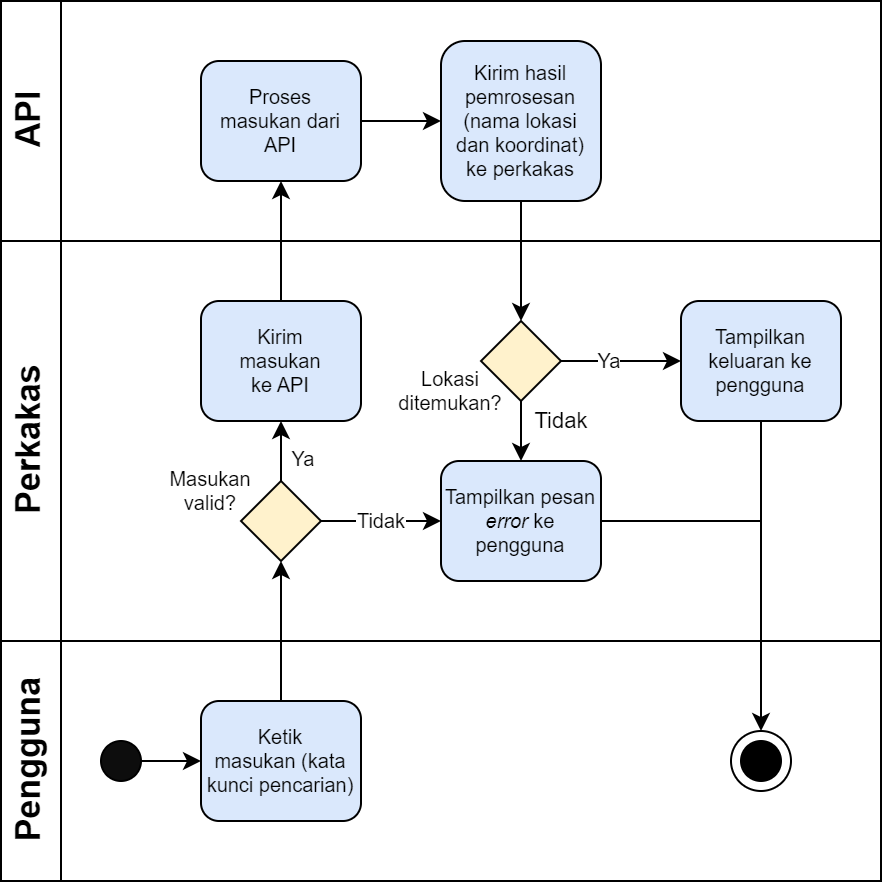
\includegraphics[width=0.55\linewidth]{diagrams-activity-searchplace}
    \caption[\textit{Activity diagram} fitur pencarian lokasi menggunakan kata kunci lokasi]{\textit{Activity diagram} dari fitur pencarian lokasi menggunakan kata kunci pencarian.}
    \label{fig:diagrams-activity-searchplace}
\end{figure}

\begin{figure}[h]
    \centering
    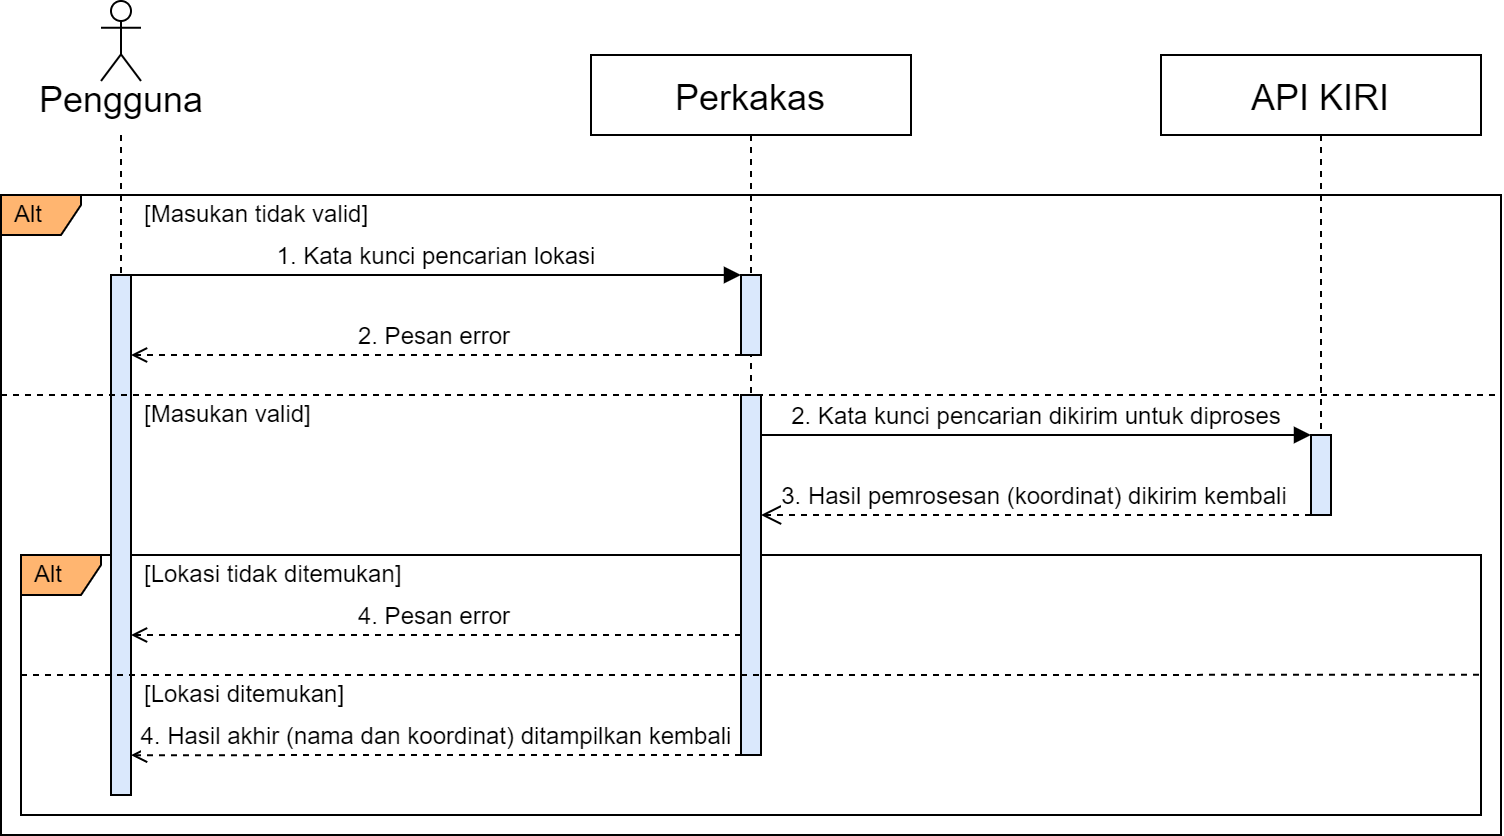
\includegraphics[width=0.8\linewidth]{diagrams-sequence-searchplace}
    \caption[\textit{Sequence diagram} fitur pencarian lokasi menggunakan kata kunci lokasi]{\textit{Sequence diagram} dari fitur pencarian lokasi menggunakan kata kunci pencarian.}
    \label{fig:diagrams-sequence-searchplace}
\end{figure}

\begin{enumerate}
	\item Perkakas akan meminta masukan dari pengguna berupa kata kunci dari lokasi yang ingin dicari.
	\item Masukan akan dicek oleh perkakas validitasnya. Dalam kasus ini, masukan hanya akan dianggap tidak valid apabila pengguna tidak memasukkan apapun sebagai masukan perkakas (masukan kosong).
	\item Jika kata kunci masukan:

	\begin{itemize}
		\item tidak valid, maka perkakas akan mengeluarkan pesan \textit{error} dan keluar.
		\item dianggap valid, kata kunci tersebut akan dikirim ke API KIRI untuk diproses lebih lanjut.
	\end{itemize}
	
	\item Setelah selesai diproses, keluaran dari API akan dikembalikan ke perkakas.
	\item Perkakas akan mengecek keluaran yang diterimanya. Apabila lokasi:
	
	\begin{itemize}
		\item ditemukan, maka nama dan koordinat \latlon lokasi akan ditampilkan ke pengguna sebagai keluaran akhir.
		\item tidak ditemukan, maka perkakas akan mengeluarkan pesan \textit{error} dan keluar.
	\end{itemize}
	
	Perlu diingat bahwa perkakas tidak peduli apakah lokasi yang ditemukan benar (sesuai dengan yang diinginkan pengguna) atau tidak.
	
\end{enumerate}

\subsection{Mencari rute dengan angkot menggunakan \latlon lokasi}
\label{sec:design-flow-findroute}

\textit{Activity} dan \textit{sequence} diagram untuk fitur pencarian rute dengan menggunakan koordinat lokasi awal dan akhir dapat dilihat di gambar \ref{fig:diagrams-activity-findroute} dan \ref{fig:diagrams-sequence-findroute}. Detail dari alur kerja untuk fitur ini adalah sebagai berikut.

\begin{figure}[h]
    \centering
    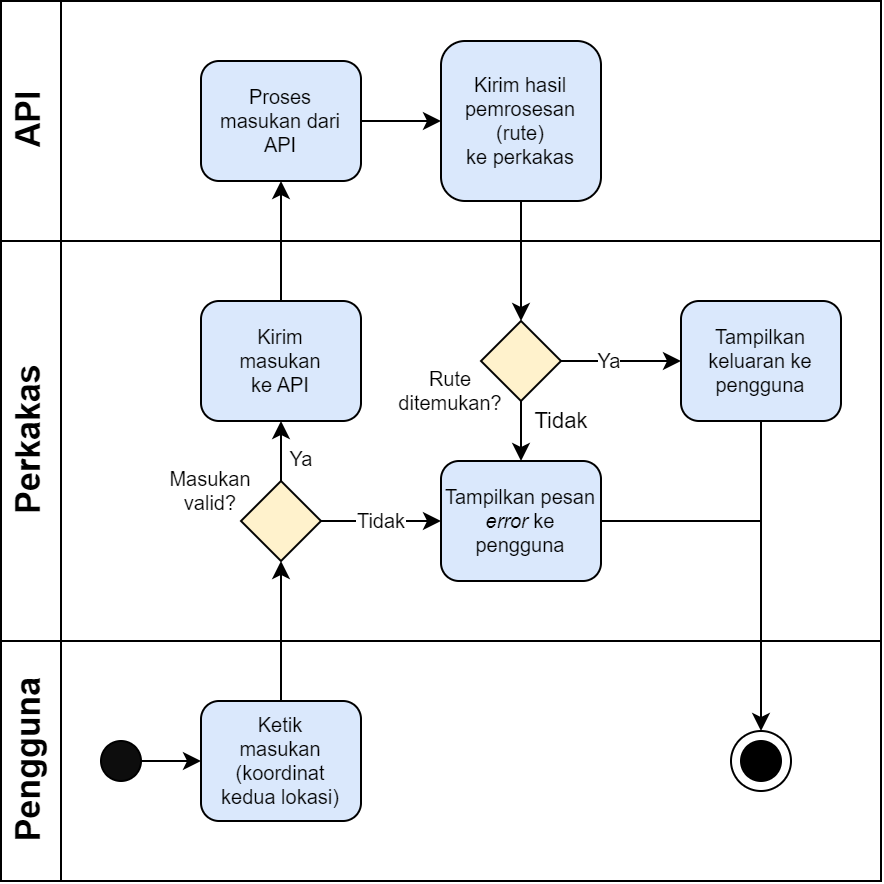
\includegraphics[width=0.55\linewidth]{diagrams-activity-findroute}
    \caption[\textit{Activity diagram} fitur pencarian rute angkot menggunakan koordinat lokasi]{\textit{Activity diagram} dari fitur pencarian rute angkot menggunakan \latlon lokasi.}
    \label{fig:diagrams-activity-findroute}
\end{figure}

\begin{figure}[h]
    \centering
    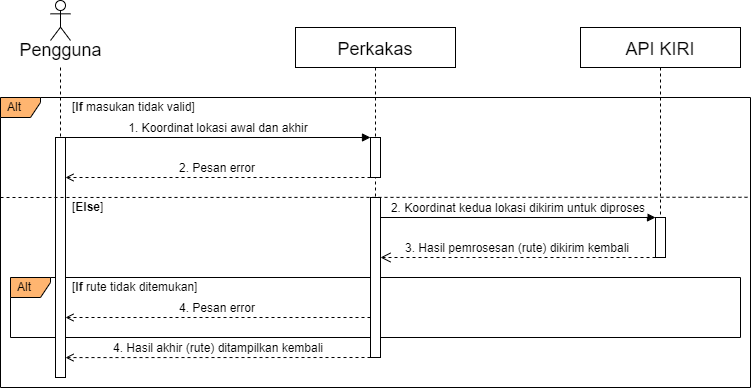
\includegraphics[width=0.8\linewidth]{diagrams-sequence-findroute}
    \caption[\textit{Sequence diagram} fitur pencarian rute angkot menggunakan koordinat lokasi]{\textit{Sequence diagram} dari fitur pencarian rute angkot menggunakan \latlon lokasi.}
    \label{fig:diagrams-sequence-findroute}
\end{figure}

\begin{enumerate}
	\item Perkakas akan meminta dua buah masukan dari pengguna, berupa koordinat \latlon dari lokasi awal (mulai) dan lokasi akhir (tujuan).
	\item Masukan akan dicek oleh perkakas validitasnya. Dalam kasus ini, masukan akan dianggap tidak valid apabila ada masukan yang bukan berupa koordinat \latlon .
	\item Jika:
	
	\begin{itemize}
		\item satu atau lebih masukan tidak valid, maka perkakas akan mengeluarkan pesan \textit{error} dan keluar.
		\item kedua masukan dianggap valid, kedua koordinat tersebut akan dikirim ke API KIRI untuk diproses lebih lanjut.
	\end{itemize}
	 
	\item Setelah selesai diproses, keluaran dari API akan dikembalikan ke perkakas.
	\item Perkakas akan mengecek keluaran yang diterimanya. Apabila rute:
	
	\begin{itemize}
		\item berhasil ditemukan (ada setidaknya satu langkah dalam rute), maka rute tersebut akan ditampilkan ke pengguna sebagai keluaran akhir.
		\item tidak berhasil ditemukan, maka perkakas akan mengeluarkan pesan \textit{error} dan keluar.
	\end{itemize}
	
\end{enumerate}

\subsection{Mencari rute dengan angkot menggunakan kata kunci pencarian lokasi}
\label{sec:design-flow-direct}

\textit{Activity} dan \textit{sequence} diagram untuk fitur pencarian rute dengan pencarian langsung lokasi awal dan akhirnya dapat dilihat di gambar \ref{fig:diagrams-activity-direct} dan \ref{fig:diagrams-sequence-direct}. Berikut alur dari diagram-diagram tersebut.

\begin{enumerate}
	\item Perkakas akan meminta masukan dari pengguna berupa kata kunci dari lokasi awal dan lokasi akhir yang ingin dicari.
	\item Masukan untuk lokasi awal akan dicek oleh perkakas validitasnya. Dalam kasus ini, masukan hanya akan dianggap tidak valid apabila pengguna tidak memasukkan apapun (masukan kosong), atau memasukkan koordinat \latlon sebagai masukan perkakas.
	\item Jika kata kunci masukan:
	
	\begin{itemize}
		\item tidak valid, maka perkakas akan mengeluarkan pesan \textit{error} dan keluar.
		\item dianggap valid, kata kunci tersebut akan dikirim ke API KIRI untuk diproses lebih lanjut.
	\end{itemize}
	 
	\item Setelah selesai diproses, keluaran dari API akan dikembalikan ke perkakas.
	\item Perkakas akan mengecek keluaran yang diterimanya. Apabila lokasi:
	
	\begin{itemize}
		\item tidak ditemukan, maka perkakas akan mengeluarkan pesan \textit{error} dan keluar.
		\item ditemukan, maka nama dan koordinat \latlon lokasi awal akan disimpan sebagai variabel untuk dipakai di langkah selanjutnya.
	\end{itemize}
	
	\item Langkah 2 sampai 5 akan diulang kembali untuk lokasi akhir.
	\item Jika kata kunci kedua lokasi berhasil diproses, perkakas akan mengirim kembali koordinat \latlon dari kedua lokasi tersebut ke API sebagai masukan untuk proses kedua, yaitu mencari rute angkot dengan koordinat \latlon lokasi.
	\item Setelah selesai diproses, keluaran berupa rute dari API akan dikembalikan ke perkakas.
	\item Perkakas akan mengecek keluaran yang diterimanya. Apabila rute:
	
	\begin{itemize}
		\item berhasil ditemukan (ada setidaknya satu langkah dalam rute), maka rute tersebut akan ditampilkan ke pengguna sebagai keluaran akhir.
		\item tidak berhasil ditemukan, maka perkakas akan mengeluarkan pesan \textit{error} dan keluar.
	\end{itemize}
	
\end{enumerate}

\begin{figure}[h]
    \centering
    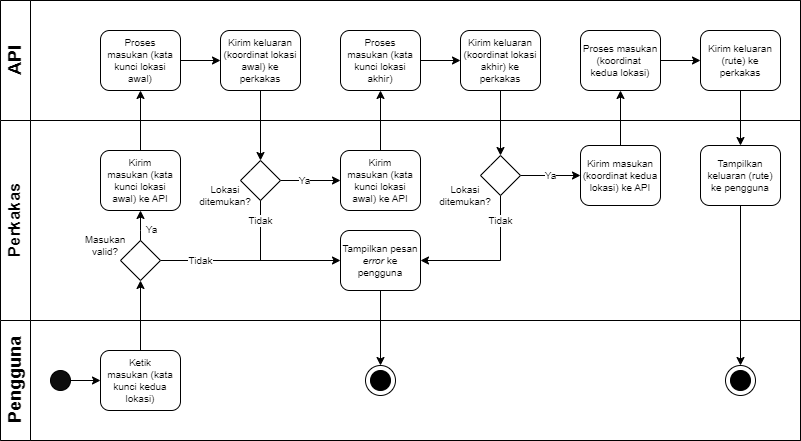
\includegraphics[width=\linewidth]{diagrams-activity-direct}
    \caption[\textit{Activity diagram} fitur pencarian rute angkot menggunakan kata kunci lokasi]{\textit{Activity diagram} dari fitur pencarian rute angkot menggunakan kata kunci pencarian.}
    \label{fig:diagrams-activity-direct}
\end{figure}

\begin{figure}[h]
    \centering
    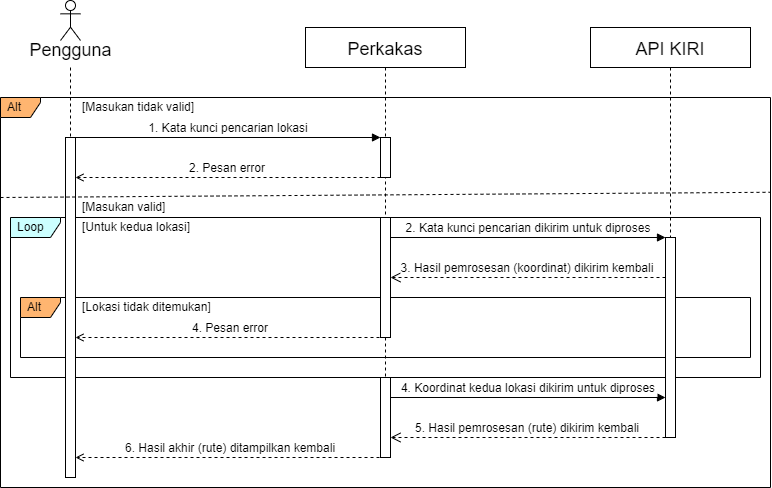
\includegraphics[width=0.8\linewidth]{diagrams-sequence-direct}
    \caption[\textit{Sequence diagram} fitur pencarian rute angkot menggunakan kata kunci lokasi]{\textit{Sequence diagram} dari fitur pencarian rute angkot menggunakan kata kunci pencarian.}
    \label{fig:diagrams-sequence-direct}
\end{figure}

\section{Rancangan Implementasi Perkakas}
\label{sec:design-implementation}

Bagian ini akan membahas hal-hal seputar rancangan implementasi alur kerja perkakas, variabel-variabel utama yang diperlukan di dalam perkakas, serta hal-hal seputar fungsi-fungsi yang ada di dalam perkakas, seperti nama fungsinya, apa tujuan dari fungsi tersebut, masukan dan keluarannya, serta garis besar dari cara kerja fungsi tersebut.

\subsection{Cara Kerja Perkakas}
\label{sec:design-implementation-overview}

Untuk setiap operasinya, perkakas \cl KIRI ini terdiri atas empat proses utama, dengan urutan operasi internal sebagai berikut.

\begin{enumerate}
	\item Penerimaan opsi dan argumen \\
	Di proses ini, perkakas akan melakukan pemeriksaan paling dasar, yaitu memeriksa apakah pengguna menggunakan opsi dan memasukkan argumennya dengan tepat atau tidak. \textit{Error checking} yang dilakukan di tahap ini juga hanya sebatas pengecekan dasar, seperti pengecekan validitas opsi yang digunakan, jumlah argumen yang dimasukkan, serta validitas mode operasi dari perkakas (opsi \verb|--mode|). Kesalahan apapun yang terdapat di hal-hal selain kedua aspek tersebut hanya akan ditandai.
	\item Verifikasi kebenaran opsi dan argumen \\
	Di proses ini, perkakas akan melakukan pengecekan lanjutan terhadap argumen-argumen yang dimasukkan pengguna. Jika ada argumen yang tidak valid, perkakas akan langsung berhenti dan mengeluarkan pesan \textit{error} yang sesuai.
	\item Pengiriman permintaan GET ke API serta penerimaan kembali respons\\
	Setelah semua opsi dan argumen yang dibutuhkan diverifikasi validitasnya, perkakas akan membangun URL yang diperlukan untuk permintaan GET ke API, dan melakukan permintaan tersebut melalui cURL. \textit{Library} cURL ini nantinya juga adalah \textit{library} yang memfasilitasi penerimaan kembali respons dari API.
	\item Verifikasi akhir respons API \\
	Terakhir, isi dari respons API akan diperiksa. Segala abnormalitas yang terdapat di dalam isi respons tersebut akan ditangani langsung oleh perkakas dalam bentuk pesan-pesan \textit{error} untuk tiap kasusnya.
\end{enumerate}

\subsection{Tipe Data Tambahan}
\label{sec:design-implementation-customtypes}

Salah satu dari variabel global yang ada di perkakas ini memiliki tipe data \verb|chunk|, yang merupakan sebuah \verb|struct| tambahan yang dibuat sendiri. Adapun variabel-variabel yang ada di dalam struktur tersebut adalah sebagai berikut.

\begin{itemize}
	\item \verb|data| (\verb|char *|)
	\item \verb|size| (\verb|size_t|)
\end{itemize}
\noindent
Struktur ini akan digunakan untuk variabel \verb|responsedata|, yang akan diisi dengan respons dari API KIRI setelah eksekusi proses cURL. Variabel \verb|data| di struktur ini merupakan penunjuk ke \textit{array} karakter yang akan menampung data dari respons API itu sendiri, sedangkan \verb|size|, yang merupakan sebuah \textit{unsigned integer}, akan diisi dengan ukuran dari data tersebut.

\subsection{Variabel Global}
\label{sec:design-implementation-globalvars}

Perkakas ini memiliki beberapa variabel global, yang sengaja diletakkan sebagai variabel global karena variabel-variabel ini digunakan di hampir keseluruhan dari keempat proses di subbab \ref{sec:design-implementation-overview}. Adapun variabel-variabel ini adalah sebagai berikut:

\begin{itemize}
	\item \verb|responsedata| (\verb|chunk|) \\
	Variabel ini akan diisi oleh respons dari API KIRI. Seperti yang telah dipaparkan secara singkat di subbab sebelumnya, struktur ini memiliki dua variabel, yaitu \verb|data|, yang akan berisi data responsnya sendiri, dan \verb|size|, yang merupakan ukuran dari data tersebut.
	\item \verb|responseJSON| (\verb|cJSON|) \\
	Berisi hasil konversi JSON dari respons API yang dapat dibaca oleh perkakas dan utilitas-utilitas \textit{library} cJSON.
	\item \verb|URL| (\verb|char[]|) \\
	Basis dari URL yang akan digunakan sebagai URL permintaan GET ke API. Awalnya variabel ini akan berisi ``\verb|https://projectkiri.id/api?version=2|''\textemdash bagian awal ini tidak akan berubah bagaimanapun permintaan GET-nya.
	\item \verb|mode| (\verb|int|) \\
	Kode operasional perkakas berupa bilangan bulat. Bilangan ini memiliki rentang dari -1 hingga 4, dengan arti dari tiap bilangan sebagai berikut.
	
	\begin{itemize}
		\item \textbf{-1}: Mode belum didefinisikan
		\item \textbf{0}: Mode tidak valid
		\item \textbf{1}: Mode bantuan (\textit{help})
		\item \textbf{2}: Mode \textit{searchplace}
		\item \textbf{3}: Mode \textit{findroute}
		\item \textbf{4}: Mode \textit{direct}
	\end{itemize}
	
	\item \verb|region| (\verb|int|) \\
	Kode region berupa bilangan bulat untuk mode \verb|searchplace|. Bilangan ini memiliki rentang dari -1 hingga 4, di mana arti dari tiap bilangan dapat dilihat di daftar berikut.
	
	\begin{itemize}
		\item \textbf{-1}: Region belum didefinisikan
		\item \textbf{0}: Region tidak valid
		\item \textbf{1}: cgk (Cengkareng/Jakarta)
		\item \textbf{2}: bdo (Bandung)
		\item \textbf{3}: mlg (Malang)
		\item \textbf{4}: sub (Surabaya)
	\end{itemize}
	
	\item \verb|query| (\verb|char[]|) \\
	\textit{String} (berupa \textit{array} karakter) yang menyimpan kata kunci pencarian lokasi untuk mode \verb|searchplace|.
	\item \verb|start| (\verb|char[]|) \\
	\textit{String} (berupa \textit{array} karakter) yang menyimpan koordinat lokasi awal (\verb|findroute|) atau kata kunci pencarian lokasi awal (\verb|direct|).
	\item \verb|finish| (\verb|char[]|) \\
	\textit{String} (berupa \textit{array} karakter) yang menyimpan koordinat lokasi akhir (\verb|findroute|) atau kata kunci pencarian lokasi akhir (\verb|direct|).
	\item \verb|escape| (\verb|char[]|) \\
	Variabel ini dibutuhkan karena pengkodean URL (untuk permintaan GET) tidak mendukung karakter spasi (` '), melainkan ``\verb|%20|''. \textit{String} yang karakter spasinya sudah diganti dengan ``\verb|%20|'' akan disimpan sementara di variabel ini, sebelum isinya disalin kembali ke variabel awalnya.
	\item \verb|regstart| (\verb|int|) \\
	Kode region lokasi awal berupa bilangan bulat untuk mode \verb|direct|. Bilangan ini memiliki rentang dari -1 hingga 4, dengan tiap bilangan bulat merepresentasikan region yang sama dengan kode bilangan untuk variabel \verb|region|.
	\item \verb|regfinish| (\verb|int|) \\
	Kode region lokasi akhir berupa bilangan bulat untuk mode \verb|direct|. Bilangan ini memiliki rentang dari -1 hingga 4, dengan tiap bilangan bulat merepresentasikan region yang sama dengan kode bilangan untuk variabel \verb|region|.
	\item \verb|locale| (\verb|int|) \\
	Kode bahasa berupa bilangan bulat. Bilangan ini memiliki rentang dari 0 hingga 2, dengan tiap-tiap bilangan merepresentasikan arti berikut.
	
	\begin{itemize}
		\item \textbf{0}: id (Indonesia)
		\item \textbf{1}: en (Inggris)
		\item \textbf{2}: Kode bahasa tidak valid
	\end{itemize}
	
	 Variabel ini juga merupakan satu-satunya variabel kode \textit{integer} yang, jika tidak diubah nilai awalnya (\textbf{0}), tidak akan menyebabkan \textit{error}.
	\item \verb|step| (\verb|int|) \\
	Kode khusus untuk mode \verb|direct| yang menandakan proses mana yang sedang \linebreak berlangsung\textemdash pencarian lokasi awal, pencarian lokasi akhir, atau pencarian rute.
	\item \verb|error| (\verb|int|) \\
	Kode yang menandakan apakah sebuah \textit{error} telah terjadi. Nilai awal dari variabel ini adalah \textbf{0}, dan jika variabel ini diganti menjadi \textbf{1}, di pengecekan kode \textit{error} selanjutnya, perkakas akan dihentikan.
\end{itemize}

\subsection{\texttt{print\char`_help()}}
\label{sec:design-code-printhelp}

Fungsi ini merupakan fungsi yang akan dipanggil ketika pengguna memilih opsi standar \verb|--help|. Keterangan singkat dari fungsi ini dapat dilihat di tabel \ref{tab:design-code-printhelp-details}.

\begin{table}[H]
    \centering
    \begin{tabular}{| l | c p{10cm} |}
	\hline
		\textbf{Nama fungsi} & \multicolumn{2}{p{10.5cm} |}{\texttt{print\char`_help()}} \\
	\hline
		\textbf{Tujuan} & \multicolumn{2}{p{10.5cm} |}{Menampilkan bantuan penggunaan perkakas.} \\
	\hline
		\textbf{\textit{Input}} & \multicolumn{2}{p{10.5cm} |}{Fungsi ini tidak memerlukan masukan apapun.} \\
	\hline
		\textbf{\textit{Output}} & \multicolumn{2}{p{10.5cm} |}{Sekumpulan array karakter yang merupakan bantuan penggunaan perkakas.} \\
	\hline
		\textbf{\textit{Pseudocode}} & \multicolumn{2}{p{10.5cm} |}{\textit{Pseudocode} fungsi ini tidak ditulis karena satu-satunya proses dalam fungsi ini adalah mengeluarkan \textit{array-array} karakter.} \\
	\hline
	\end{tabular}
    \caption{Detail dari fungsi \texttt{print\char`_help()}.}
    \label{tab:design-code-printhelp-details}
\end{table}

\subsection{\texttt{replace\char`_space()}}
\label{sec:design-code-replacespace}

Fungsi ini merupakan fungsi yang berguna untuk meng-\textit{escape} semua karakter spasi (` ') dalam variabel-variabel kata kunci pencarian sebelum isi dari variabel-variabel tersebut dimasukkan ke dalam URL untuk permintaan GET. Hal ini perlu dilakukan karena pengkodean HTML yang digunakan untuk format URL tidak medukung karakter spasi, dan melainkan mensubstitusi seluruh kejadian karakter tersebut dalam suatu URL menjadi `\%20'. Fungsi ini akan menerima sebuah \textit{array} karakter berisi URL permintaan sebagai masukannya, mengganti semua karakter spasi yang ada di dalamnya menjadi `\%20', dan meletakkan hasilnya di variabel global \verb|escape|. Adapun keterangan singkat dari fungsi ini dapat dilihat di tabel \ref{tab:design-code-printhelp-details}.

\begin{table}[H]
    \centering
    \begin{tabular}{| l | c p{10cm} |}
	\hline
		\textbf{Nama fungsi} & \multicolumn{2}{p{10.5cm} |}{\texttt{replace\char`_space()}} \\
	\hline
		\textbf{Tujuan} & \multicolumn{2}{p{10.5cm} |}{Meng-\textit{escape} seluruh karakter spasi di \textit{string} masukan.} \\
	\hline
		\textbf{\textit{Input}} & \multicolumn{2}{p{10.5cm} |}{Sebuah \textit{string} berupa \textit{array} karakter.} \\
	\hline
		\textbf{\textit{Output}} & \multicolumn{2}{p{10.5cm} |}{String tersebut yang sudah di-\textit{escape} karakter spasinya, dimasukkan ke variabel global \texttt{escape}.} \\
	\hline
		\textbf{\textit{Pseudocode}} & \multicolumn{2}{p{10.5cm} |}{Lihat di algoritma \ref{alg:design-replacespace}.} \\
	\hline
	\end{tabular}
    \caption{Detail dari fungsi \texttt{replace\char`_space()}.}
    \label{tab:design-code-replacespace-details}
\end{table}

\begin{algorithm}[h]
	\caption{Algoritma fungsi \texttt{replace\char`_space()}}
	\label{alg:design-replacespace}
	% input & output
	\vspace{-0.6\baselineskip}
	\begin{flushleft}
		Catatan: Karakter \textquotesingle *\textquotesingle\xspace berarti variabel tersebut merupakan variabel global.\\
        \textbf{Input:} $string$ \\
        \textbf{Output:} $escape$* \\
	\end{flushleft}
	\vspace{-1.05\baselineskip}
	\begin{algorithmic}
		\State $j \gets 0$
		\For{$i \gets 0$ \textbf{to} size of $string$}
			\If{$string[i]$ == \textquotesingle\textbackslash 0\textquotesingle} \Comment{Berhenti jika fungsi sudah mencapai karakter terakhir $string$}
			    \State break 
			\EndIf
		
			\If{$string[i]$ == \textquotesingle\xspace\textquotesingle}
			    \State $escape[j] \gets$ \textquotesingle\%\textquotesingle
			    \State $escape[j + 1] \gets$ \textquotesingle 2\textquotesingle
			    \State $escape[j + 2] \gets$ \textquotesingle 0\textquotesingle
			    \State $j \gets j + 2$ \Comment{Majukan indeks $escape$ sebanyak 3 (2 + 1 di akhir fungsi)}
			\Else
				\State $escape[j] \gets string[i]$ 
			\EndIf
			\State $j \gets j + 1$
		\EndFor
	\end{algorithmic}
\end{algorithm}

\subsection{\texttt{build\char`_url\char`_searchplace()}}
\label{sec:design-code-buildurl-searchplace}

Fungsi ini merupakan fungsi yang digunakan untuk pembangunan URL permintaan	GET untuk proses pencarian lokasi. Keterangan dari fungsi ini dapat dilihat di tabel \ref{tab:design-code-buildurl-searchplace-details}.
	
	Selain itu, fitur ini juga memiliki implementasi tambahan yang tidak ada di API KIRI, yaitu implementasi variabel \verb|locale| untuk fitur pencarian lokasi, yang memungkinkan pemilihan bahasa Indonesia (\verb|id|) atau Inggris (\verb|en|) untuk keluaran serta pesan-pesan \textit{error} yang berhubungan dengan proses tersebut.

\begin{table}[H]
    \centering
    \begin{tabular}{| l | c p{10cm} |}
	\hline
		\textbf{Nama fungsi} & \multicolumn{2}{p{10.5cm} |}{\texttt{build\char`_url\char`_searchplace()}} \\
	\hline
		\textbf{Tujuan} & \multicolumn{2}{p{10.5cm} |}{Membangun URL untuk permintaan GET pencarian lokasi ke API KIRI.} \\
	\hline
		\textbf{\textit{Input}} & - & \texttt{locale}: Kode bahasa \\
		 & - & \texttt{region}: Region dari lokasi yang ingin dicari \\
		 & - & \texttt{query}: Kata kunci pencarian lokasi \\
	\hline
		\textbf{\textit{Output}} & - & \texttt{error} (variabel global) \\
		 & - & \texttt{url} (variabel global) \\
	\hline
		\textbf{\textit{Pseudocode}} & \multicolumn{2}{p{10.5cm} |}{Lihat di algoritma \ref{alg:design-buildurl-searchplace}.} \\
	\hline
	\end{tabular}
    \caption{Detail dari fungsi \texttt{build\char`_url\char`_searchplace()}.}
    \label{tab:design-code-buildurl-searchplace-details}
\end{table}

\begin{algorithm}[h]
	\caption{Algoritma fungsi \texttt{build\char`_url\char`_searchplace()}}
	\label{alg:design-buildurl-searchplace}
	% input & output
	\vspace{-0.6\baselineskip}
	\begin{flushleft}
		Catatan: Karakter \textquotesingle *\textquotesingle\xspace berarti variabel tersebut merupakan variabel global.\\
        \textbf{Input:} $locale$, $region$, $query$ \\
        \textbf{Output:} $url$*, $error$* \\
	\end{flushleft}
	\vspace{-1.05\baselineskip}
	\begin{algorithmic}
		\If{$locale$ == 2}
		    \State $error \gets 1$
			\State \textit{print} pesan \textit{error}: $locale$ tidak valid
			\State hentikan perkakas
		\EndIf
		
		\Switch{$region$}
			\Case{$-1$}
				\State $error \gets 1$
				\State \textit{print} pesan \textit{error} sesuai $locale$: $region$ tidak dimasukkan
				\State hentikan perkakas
			\EndCase
			\Case{$1$}
				\State tambahkan parameter $region$ \textquotesingle\textquotesingle cgk\textquotesingle\textquotesingle\xspace ke $url$
				\State break
			\EndCase
			\Case{$2$}
				\State tambahkan parameter $region$ \textquotesingle\textquotesingle bdo\textquotesingle\textquotesingle\xspace ke $url$
				\State break
			\EndCase
			\Case{$3$}
				\State tambahkan parameter $region$ \textquotesingle\textquotesingle mlg\textquotesingle\textquotesingle\xspace ke $url$
				\State break
			\EndCase
			\Case{$4$}
				\State tambahkan parameter $region$ \textquotesingle\textquotesingle sub\textquotesingle\textquotesingle\xspace ke $url$
				\State break
			\EndCase
			\Default
				\State $error \gets 1$
				\State \textit{print} pesan \textit{error} sesuai $locale$: $region$ tidak valid
				\State hentikan perkakas
			\EndDefault
		\EndSwitch
		
		\If{$query$ == \textquotesingle\textbackslash 0\textquotesingle}
		    \State $error \gets 1$
			\State \textit{print} pesan \textit{error} sesuai $locale$: $query$ tidak dimasukkan
			\State hentikan perkakas
		\Else
			\State tambahkan parameter $query$ ke $url$
		\EndIf
		
		\State tambahkan parameter kunci API ke $url$
	\end{algorithmic}
\end{algorithm}

\subsection{\texttt{build\char`_url\char`_findroute()}}
\label{sec:design-code-buildurl-findroute}

Fungsi ini merupakan fungsi yang digunakan untuk pembangunan URL permintaan	GET untuk proses pencarian rute angkot. Adapun penjelasan dari fungsi ini dapat dilihat di tabel \ref{tab:design-code-buildurl-findroute-details}.

\begin{table}[H]
    \centering
    \begin{tabular}{| l | c p{10cm} |}
	\hline
		\textbf{Nama fungsi} & \multicolumn{2}{p{10.5cm} |}{\texttt{build\char`_url\char`_findroute()}} \\
	\hline
		\textbf{Tujuan} & \multicolumn{2}{p{10.5cm} |}{Membangun URL untuk permintaan GET pencarian rute ke API KIRI.} \\
	\hline
		\textbf{\textit{Input}} & - & \texttt{locale} (variabel global) \\
		 & - & \texttt{start}: Koordinat lokasi awal \\
		 & - & \texttt{finish}: Koordinat lokasi akhir \\
	\hline
		\textbf{\textit{Output}} & - & \texttt{error} (variabel global) \\
		 & - & \texttt{url} (variabel global) \\
	\hline
		\textbf{\textit{Pseudocode}} & \multicolumn{2}{p{10.5cm} |}{Lihat di algoritma \ref{alg:design-buildurl-findroute}.} \\
	\hline
%		\textbf{Skenario utama} & 1. & Perkakas membaca masukan berupa kata kunci pencarian lokasi dari argumen dalam perintah \cl. \\
%		 & 2. & Perkakas memproses masukan tersebut dan mengirimkannya ke API KIRI untuk diproses lebih lanjut. \\
%    \hline
	\end{tabular}
    \caption{Detail dari fungsi \texttt{build\char`_url\char`_findroute()}.}
    \label{tab:design-code-buildurl-findroute-details}
\end{table}

\begin{algorithm}[h]
	\caption{Algoritma fungsi \texttt{build\char`_url\char`_findroute()}}
	\label{alg:design-buildurl-findroute}
	% input & output
	\vspace{-0.6\baselineskip}
	\begin{flushleft}
		Catatan: Karakter \textquotesingle *\textquotesingle\xspace berarti variabel tersebut merupakan variabel global.\\
		\textbf{Variabel global:}  \\
        \textbf{Input:} $locale$, $start$, $finish$ \\
        \textbf{Output:} $url$*, $error$* \\
	\end{flushleft}
	\vspace{-1.05\baselineskip}
	\begin{algorithmic}
	
		\Switch{$region$}
			\Case{$1$}
			    \State tambahkan parameter $locale$ \textquotesingle\textquotesingle en\textquotesingle\textquotesingle\xspace ke $url$
				\State break
			\EndCase
			\Case{$2$}
			    \State $error \gets 1$
				\State \textit{print} pesan \textit{error}: $locale$ tidak valid
				\State hentikan perkakas
			\EndCase
			\Default
				\State tambahkan parameter $locale$ \textquotesingle\textquotesingle id\textquotesingle\textquotesingle\xspace ke $url$
				\State break
			\EndDefault
		\EndSwitch
		
		\If{$start$ == \textquotesingle\textbackslash 0\textquotesingle}
		    \State $error \gets 1$
			\State \textit{print} pesan \textit{error} sesuai $locale$: $start$ tidak dimasukkan
			\State hentikan perkakas
		\Else
			\State tambahkan parameter $start$ ke $url$
		\EndIf
		
		\If{$finish$ == \textquotesingle\textbackslash 0\textquotesingle}
		    \State $error \gets 1$
			\State \textit{print} pesan \textit{error} sesuai $locale$: $finish$ tidak dimasukkan
			\State hentikan perkakas
		\Else
			\State tambahkan parameter $query$ ke $url$
		\EndIf
		
		\State tambahkan parameter presentation \textquotesingle\textquotesingle desktop\textquotesingle\textquotesingle\xspace ke $url$
		\State tambahkan parameter kunci API ke $url$
	\end{algorithmic}
\end{algorithm}

\subsection{\texttt{reset\char`_url()}}
\label{sec:design-code-buildurl-reset}

Fungsi ini digunakan untuk mengembalikan isi dari variabel \verb|URL| ke nilai semula, dengan cara \mbox{mengganti} isi dari variabel tersebut kembali ke nilai awalnya, yaitu ``\verb|https://projectkiri.id/|\linebreak\verb|api?version=2|''. Penjelasan singkat dari fungsi ini terdapat di tabel \ref{tab:design-code-buildurl-reset-details}.

\begin{table}[H]
    \centering
    \begin{tabular}{| l | c p{10cm} |}
	\hline
		\textbf{Nama fungsi} & \multicolumn{2}{p{10.5cm} |}{\texttt{reset\char`_url()}} \\
	\hline
		\textbf{Tujuan} & \multicolumn{2}{p{10.5cm} |}{Mengembalikan URL ke bentuk umumnya.} \\
	\hline
		\textbf{\textit{Input}} & \multicolumn{2}{p{10.5cm} |}{\texttt{url} (variabel global)} \\
	\hline
		\textbf{\textit{Output}} & \multicolumn{2}{p{10.5cm} |}{\texttt{url} yang sudah dikembalikan nilainya} \\
	\hline
		\textbf{\textit{Pseudocode}} & \multicolumn{2}{p{10.5cm} |}{\textit{Pseudocode} fungsi ini tidak ditulis karena fungsi ini hanya berisi satu buah proses penggantian nilai \textit{array} karakter.} \\
	\hline
%		\textbf{Skenario utama} & 1. & Perkakas membaca masukan berupa kata kunci pencarian lokasi dari argumen dalam perintah \cl. \\
%		 & 2. & Perkakas memproses masukan tersebut dan mengirimkannya ke API KIRI untuk diproses lebih lanjut. \\
%    \hline
	\end{tabular}
    \caption{Detail dari fungsi \texttt{reset\char`_url()}.}
    \label{tab:design-code-buildurl-reset-details}
\end{table}

\subsection{\texttt{execute\char`_curl()}}
\label{sec:design-code-curl-execute}

Fungsi ini digunakan untuk proses pengiriman permintaan ke API, serta penerimaan respons dari API. Semua utilitas dari library cURL yang dipakai dalam perkakas ini, seperti \textit{handler} kelebihan memori data yang masuk, dan aturan variabel apa yang akan diisi dengan data respons API, akan diimplementasikan hanya di dalam fungsi ini. Adapun keterangan singkat dari fungsi ini tertera di tabel \ref{tab:design-code-curl-execute}.

\begin{table}[H]
    \centering
    \begin{tabular}{| l | c p{10cm} |}
	\hline
		\textbf{Nama fungsi} & \multicolumn{2}{p{10.5cm} |}{\texttt{execute\char`_curl()}} \\
	\hline
		\textbf{Tujuan} & \multicolumn{2}{p{10.5cm} |}{Menjalankan proses cURL.} \\
	\hline
		\textbf{\textit{Input}} & - & \texttt{responsedata} (variabel global) \\
		 & - & \texttt{mode} (variabel global) \\
		 & - & \texttt{step} (variabel global) \\
	\hline
		\textbf{\textit{Output}} & \multicolumn{2}{p{10.5cm} |}{\texttt{responsedata} yang sudah diisi dengan data respons cURL} \\
	\hline
		\textbf{\textit{Pseudocode}} & \multicolumn{2}{p{10.5cm} |}{Lihat algoritma \ref{alg:design-curl-execute}.} \\
	\hline
%		\textbf{Skenario utama} & 1. & Perkakas membaca masukan berupa kata kunci pencarian lokasi dari argumen dalam perintah \cl. \\
%		 & 2. & Perkakas memproses masukan tersebut dan mengirimkannya ke API KIRI untuk diproses lebih lanjut. \\
%    \hline
	\end{tabular}
    \caption{Detail dari fungsi \texttt{execute\char`_curl()}.}
    \label{tab:design-code-curl-execute}
\end{table}

\begin{algorithm}[h]
	\caption{Algoritma fungsi \texttt{execute\char`_curl()}}
	\label{alg:design-curl-execute}
	% input & output
	\vspace{-0.6\baselineskip}
	\begin{flushleft}
		Catatan: Karakter \textquotesingle *\textquotesingle\xspace berarti variabel tersebut merupakan variabel global.\\
		\textbf{Input:} $responsedata$*, $mode$*, $step$* \\
		\textbf{Output:} $responsedata$* \\
	\end{flushleft}
	\vspace{-1.05\baselineskip}
	\begin{algorithmic}
		\State $curl \gets$ penunjuk ke \textit{handle} cURL
		\State $curlcode \gets$ kode respons cURL
		\State kosongkan $responsedata$ \Comment{Untuk fungsi dengan banyak langkah}
		\State inisialisasi $curl$
		
		\If{$curl \neq false$} \Comment{Selama proses cURL masih berjalan}
			\State atur opsi-opsi $curl$
			\State $curlcode \gets$ jalankan proses $curl$
			\If{$curlcode$ bukan error}
				\State \textbf{panggil fungsi:} \texttt{print\char`_curl\char`_error()}
			\EndIf
		
			\Switch{$mode$}
				\Case{$2$}
				    \State \textbf{panggil fungsi:} \texttt{write\char`_searchplace()}
					\State break
				\EndCase
				\Case{$3$}
					\State\textbf{panggil fungsi:} \texttt{write\char`_findroute()}
					\State break
				\EndCase
				\Case{$4$}
					\If{$step == 0$\xspace||\xspace$step == 1$} \Comment{Pencarian lokasi awal dan akhir}
						\State \textbf{panggil fungsi:} \texttt{write\char`_searchplace\char`_noreturns()}
						\State break
					\ElsIf{$step == 2$} \Comment{Pencarian rute}
						\State\textbf{ panggil fungsi:} \texttt{write\char`_findroute()}
						\State break
					\EndIf
				\EndCase
			\EndSwitch
			
			\State lakukan \textit{cleanup handle} $curl$
		\EndIf
		
		\State lakukan \textit{global cleanup} cURL
	\end{algorithmic}
\end{algorithm}

\subsection{\texttt{print\char`_curl\char`_error()}}
\label{sec:design-code-curl-error}

Fungsi ini merupakan fungsi sederhana yang akan mengeluarkan pesan \textit{error} apabila terjadi \textit{error} koneksi ketika perkakas ingin melakukan komunikasi dengan API KIRI. Penjelasan lebih menyeluruh untuk fungsi ini ada di tabel \ref{tab:design-code-curl-error}.

\begin{table}[H]
    \centering
    \begin{tabular}{| l | c p{10cm} |}
	\hline
		\textbf{Nama fungsi} & \multicolumn{2}{p{10.5cm} |}{\texttt{print\char`_curl\char`_error()}} \\
	\hline
		\textbf{Tujuan} & \multicolumn{2}{p{10.5cm} |}{Mengeluarkan pesan \textit{error} untuk kegagalan dalam proses cURL.} \\
	\hline
		\textbf{\textit{Input}} & \multicolumn{2}{p{10.5cm} |}{\texttt{error} (variabel global)} \\
	\hline
		\textbf{\textit{Output}} & \multicolumn{2}{p{10.5cm} |}{Pesan \textit{error} yang memberitahu pengguna bahwa telah terjadi \textit{error} dalam proses cURL.} \\
	\hline
		\textbf{\textit{Pseudocode}} & \multicolumn{2}{p{10.5cm} |}{Lihat algoritma \ref{alg:design-curl-error}.} \\
	\hline
%		\textbf{Skenario utama} & 1. & Perkakas membaca masukan berupa kata kunci pencarian lokasi dari argumen dalam perintah \cl. \\
%		 & 2. & Perkakas memproses masukan tersebut dan mengirimkannya ke API KIRI untuk diproses lebih lanjut. \\
%    \hline
	\end{tabular}
    \caption{Detail dari fungsi \texttt{print\char`_curl\char`_error()}.}
    \label{tab:design-code-curl-error}
\end{table}

\begin{algorithm}[h]
	\caption{Algoritma fungsi \texttt{print\char`_curl\char`_error()}}
	\label{alg:design-curl-error}
	% input & output
	\vspace{-0.6\baselineskip}
	\begin{flushleft}
		Catatan: Karakter \textquotesingle *\textquotesingle\xspace berarti variabel tersebut merupakan variabel global.\\
		\textbf{Input:} $error$* \\
		\textbf{Output:} Pesan \textit{error} terjadinya \textit{error} cURL \\
	\end{flushleft}
	\vspace{-1.05\baselineskip}
	\begin{algorithmic}
		\If{$error == 1$}
			\State \textit{print} pesan \textit{error} sesuai $locale$: telah terjadi error cURL
		\EndIf
	\end{algorithmic}
\end{algorithm}

\subsection{\texttt{write\char`_memalloc()}}
\label{sec:design-code-write-memalloc}

Fungsi ini adalah fungsi tambahan untuk cURL yang bertugas menerima data yang masuk dari API. Di fungsi ini juga diimplementasikan sebuah \textit{handler} pengalokasian memori, yang akan menghindari terjadinya \textit{error} akibat ukuran data yang diterima melebihi alokasi memori yang diperbolehkan untuk variabel yang akan diisi dengan data tersebut. Adapun alur kerja dari fungsi ini dapat dilihat di algoritma \ref{alg:design-write-memalloc}.

\begin{table}[H]
    \centering
    \begin{tabular}{| l | c p{10cm} |}
	\hline
		\textbf{Nama fungsi} & \multicolumn{2}{p{10.5cm} |}{\texttt{write\char`_memalloc()}} \\
	\hline
		\textbf{Tujuan} & - & Mengurus penerimaan data dari hasil proses cURL. \\
		 & - & Mencegah \textit{error} akibat kegagalan alokasi memori data yang diterima. \\
	\hline
		\textbf{\textit{Input}} & - & \texttt{incomingdata}: Variabel sementara data yang diterima \\
		 & - & \texttt{size}: Ukuran dari satu \textit{block} data \\
		 & - & \texttt{nmenb}: Berapa banyak \textit{block} data yang diterima \\
		 & - & \texttt{userdata}: Variabel yang diisi dengan data yang diterima \\
	\hline
		\textbf{\textit{Output}} & \multicolumn{2}{p{10.5cm} |}{\texttt{realsize}: Untuk verifikasi keutuhan data yang diterima} \\
	\hline
		\textbf{\textit{Pseudocode}} & \multicolumn{2}{p{10.5cm} |}{Lihat algoritma \ref{alg:design-write-memalloc}.} \\
	\hline
%		\textbf{Skenario utama} & 1. & Perkakas membaca masukan berupa kata kunci pencarian lokasi dari argumen dalam perintah \cl. \\
%		 & 2. & Perkakas memproses masukan tersebut dan mengirimkannya ke API KIRI untuk diproses lebih lanjut. \\
%    \hline
	\end{tabular}
    \caption{Detail dari fungsi \texttt{write\char`_memalloc()}.}
    \label{tab:design-write-memalloc}
\end{table}

\begin{algorithm}[h]
	\caption{Algoritma fungsi \texttt{write\char`_memalloc()}}
	\label{alg:design-write-memalloc}
	% input & output
	\vspace{-0.6\baselineskip}
	\begin{flushleft}
		\textbf{Input:} $incomingdata$, $size$, $nmenb$, $userdata$ \\
		\textbf{Output:} $realsize$ \\
	\end{flushleft}
	\vspace{-1.05\baselineskip}
	\begin{algorithmic}
		\State $realsize \gets size * nmemb$ \Comment{Hitung ukuran data yang diterima} 
		\State $memory \gets userdata$ \Comment{Masukkan data yang diterima ke variabel tujuan}
		\State $ptr \gets$ realokasi ukuran memori dari data dalam $memory$
		
		\If{$ptr ==$ NULL} \Comment{Kalau realokasi gagal...}
			\State \textit{print} pesan \textit{error}: Memori habis
			\State \textbf{return} $0$ \Comment{Menandakan bahwa realokasi memori gagal}
		\EndIf
		
		\State Isi data dalam $ptr$ ke \textit{chunk} $memory$
		\State Perbarui ukuran data dalam \textit{chunk} $memory$
		
		\State \textbf{return} $realsize$ \Comment{Untuk verifikasi keutuhan data asli}
	\end{algorithmic}
\end{algorithm}

\subsection{\texttt{write\char`_searchplace()}}
\label{sec:design-code-write-searchplace}

Fungsi ini adalah fungsi yang bertugas untuk memproses respons dari API untuk fitur pencarian lokasi dari mode \verb|searchplace|. Penjelasan singkat dari fungsi ini tertera di tabel \ref{tab:design-write-searchplace}.

\begin{table}[H]
    \centering
    \begin{tabular}{| l | c p{10cm} |}
	\hline
		\textbf{Nama fungsi} & \multicolumn{2}{p{10.5cm} |}{\texttt{write\char`_searchplace()}} \\
	\hline
		\textbf{Tujuan} & \multicolumn{2}{p{10.5cm} |}{Memproses respons API untuk fitur pencarian lokasi dan\linebreak menampilkan hasilnya ke pengguna.} \\
	\hline
		\textbf{\textit{Input}} & - & \texttt{responsedata} (variabel global) \\
		 & - & \texttt{responseJSON} (variabel global) \\
		 & - & \texttt{error} (variabel global) \\
		 & - & \texttt{locale} (variabel global) \\
	\hline
		\textbf{\textit{Output}} & \multicolumn{2}{p{10.5cm} |}{Keluaran akhir perkakas untuk mode \textit{searchplace}} \\
	\hline
		\textbf{\textit{Pseudocode}} & \multicolumn{2}{p{10.5cm} |}{Lihat algoritma \ref{alg:design-write-searchplace}.} \\
	\hline
%		\textbf{Skenario utama} & 1. & Perkakas membaca masukan berupa kata kunci pencarian lokasi dari argumen dalam perintah \cl. \\
%		 & 2. & Perkakas memproses masukan tersebut dan mengirimkannya ke API KIRI untuk diproses lebih lanjut. \\
%    \hline
	\end{tabular}
    \caption{Detail dari fungsi \texttt{write\char`_searchplace()}.}
    \label{tab:design-write-searchplace}
\end{table}

\begin{algorithm}[h]
	\caption{Algoritma fungsi \texttt{write\char`_searchplace()}}
	\label{alg:design-write-searchplace}
	% input & output
	\vspace{-0.6\baselineskip}
	\begin{flushleft}
		Catatan: Karakter \textquotesingle *\textquotesingle\xspace berarti variabel tersebut merupakan variabel global. \\
		\textbf{Input:} $responsedata$*, $responseJSON$*, $error$*, $locale$* \\
		\textbf{Output:} Keluaran akhir fitur pencarian lokasi \\
	\end{flushleft}
	\vspace{-1.05\baselineskip}
	\begin{algorithmic}
		\State $responseJSON \gets$ data dalam $responsedata$
		\State $status \gets$ \textquotesingle\textquotesingle status\textquotesingle\textquotesingle\xspace dalam $responseJSON$
		
		\If{$status \neq$ \textquotesingle\textquotesingle ok\textquotesingle\textquotesingle}
			\State $error \gets 1$
			\State \textit{print} pesan \textit{error} sesuai $locale$: hasil API \textit{error}
		\Else
			\State $result \gets$ \textquotesingle\textquotesingle searchresult\textquotesingle\textquotesingle\xspace dalam $responseJSON$
			
			\If{size of $result ==$ 0}
				\State $error \gets 1$
				\State \textit{print} pesan \textit{output} sesuai $locale$: Tidak ada lokasi yang ditemukan
			\Else
				\State $indexitem \gets 1$
				
				\ForEach{$resultitem$ \textbf{in} $result$} \Comment{Untuk setiap lokasi dalam $reesult$...}
					\State $resultitemname \gets$ \textquotesingle\textquotesingle placename\textquotesingle\textquotesingle\xspace dalam $resultitem$
					\State $resultitemlocation \gets$ \textquotesingle\textquotesingle location\textquotesingle\textquotesingle\xspace dalam $resultitem$
					\State \textit{print} $resultitemname$ dan $resultitemlocation$
					\State $indexitem \gets indexitem + 1$
				\EndFor
			\EndIf
		\EndIf
	\end{algorithmic}
\end{algorithm}
	
\subsection{\texttt{write\char`_findroute()}}
\label{sec:design-code-write-findroute}

Fungsi ini adalah fungsi yang bertugas untuk memproses respons dari API untuk fitur pencarian rute angkot. Perlu diperhatikan bahwa ada sebuah \textit{bug} dari API KIRI di mana durasi rute dalam menit tidak diterjemahkan dari bahasa Inggris, apabila variabel \verb|locale| diatur ke bahasa Indonesia. Potongan kode untuk mengatasi \textit{bug} ini juga akan terdapat di dalam fungsi ini. Adapun penjelasan lebih lanjut dari fungsi ini dapat dilihat di tabel \ref{tab:design-write-findroute}.

\begin{table}[H]
    \centering
    \begin{tabular}{| l | c p{10cm} |}
	\hline
		\textbf{Nama fungsi} & \multicolumn{2}{p{10.5cm} |}{\texttt{write\char`_findroute()}} \\
	\hline
		\textbf{Tujuan} & \multicolumn{2}{p{10.5cm} |}{Memproses respons API untuk fitur pencarian rute dan\linebreak menampilkan hasilnya ke pengguna.} \\
	\hline
		\textbf{\textit{Input}} & - & \texttt{responsedata} (variabel global) \\
		 & - & \texttt{responseJSON} (variabel global) \\
		 & - & \texttt{error} (variabel global) \\
		 & - & \texttt{locale} (variabel global) \\
	\hline
		\textbf{\textit{Output}} & \multicolumn{2}{p{10.5cm} |}{Keluaran akhir perkakas untuk mode \textit{findroute}} \\
	\hline
		\textbf{\textit{Pseudocode}} & \multicolumn{2}{p{10.5cm} |}{Lihat algoritma \ref{alg:design-write-findroute}.} \\
	\hline
%		\textbf{Skenario utama} & 1. & Perkakas membaca masukan berupa kata kunci pencarian lokasi dari argumen dalam perintah \cl. \\
%		 & 2. & Perkakas memproses masukan tersebut dan mengirimkannya ke API KIRI untuk diproses lebih lanjut. \\
%    \hline
	\end{tabular}
    \caption{Detail dari fungsi \texttt{write\char`_findroute()}.}
    \label{tab:design-write-findroute}
\end{table}

\begin{algorithm}[h]
	\caption{Algoritma fungsi \texttt{write\char`_findroute()}}
	\label{alg:design-write-findroute}
	% input & output
	\vspace{-0.6\baselineskip}
	\begin{flushleft}
		Catatan: Karakter \textquotesingle *\textquotesingle\xspace berarti variabel tersebut merupakan variabel global. \\
		\textbf{Input:} $responsedata$*, $responseJSON$*, $error$*, $locale$* \\
		\textbf{Output:} Keluaran akhir fitur pencarian rute \\
	\end{flushleft}
	\vspace{-1.05\baselineskip}
	\begin{algorithmic}
		\State $responseJSON \gets$ data dalam $responsedata$
		\State $status \gets$ \textquotesingle\textquotesingle status\textquotesingle\textquotesingle\xspace dalam $responseJSON$
		
		\If{$status \neq$ \textquotesingle\textquotesingle ok\textquotesingle\textquotesingle}
			\State $error \gets 1$
			\State \textit{print} pesan \textit{error} sesuai $locale$: hasil API \textit{error}
		\Else
			\State $result \gets$ \textquotesingle\textquotesingle routingresults\textquotesingle\textquotesingle\xspace dalam $responseJSON$
			\State $indexroute \gets 1$
			
			\ForEach{$route$ \textbf{in} $result$} \Comment{Untuk setiap rute dalam $reesult$...}
				\State $routesteps \gets$ \textquotesingle\textquotesingle steps\textquotesingle\textquotesingle\xspace dalam $resultitem$
				\State $routetime \gets$ \textquotesingle\textquotesingle traveltime\textquotesingle\textquotesingle\xspace dalam $resultitem$
				
				\If{$routetime ==$ NULL}
					\State $error \gets 1$
					\State \textit{print} pesan \textit{output} sesuai $locale$: Tidak ada rute yang ditemukan
				\Else
					\State $indexstep \gets 1$
					\If{$locale \neq 1$} \Comment{Betulkan bug durasi menit dalam $locale$ id}
						\State $routetimestring \gets$ hasil terjemahan ``minute'' dalam $routetime$ ke ``menit''
					\Else
						\State $routetimestring \gets routetime$
					\EndIf
					\State \textit{print} $routetimestring$
					
					\ForEach{$routestepitem$ \textbf{in} $routesteps$} \Comment{Untuk setiap langkah rute...}
						\State $routestepdetail \gets routestepitem[3]$ \\ \Comment{Langkah dalam bahasa natural ada di indeks ke-3}
						\State \textit{print $routestepdetail$}
					\EndFor
				\EndIf
				\State $indexroute \gets indexroute + 1$
			\EndFor
		\EndIf
	\end{algorithmic}
\end{algorithm}

\subsection{\texttt{write\char`_searchplace\char`_noreturns()}}
\label{sec:design-code-write-searchplacenoreturns}

Fungsi ini adalah fungsi yang bertugas untuk memproses respons dari API untuk fitur pencarian lokasi dari mode \verb|direct|. Berbeda dengan fungsi \verb|searchplace| sebelumnya, fungsi ini akan mengambil data dari variabel \verb|responsedata|, tetapi hanya akan menampilkan nama lokasi pertama yang ditemukan, atau jika terjadi \textit{error} di salah satu prosesnya, maka fitur ini akan menampilkan pesan \textit{error} yang sesuai. Adapun penjelasan lebih lanjut dari fungsi ini dapat dilihat di tabel \ref{tab:design-write-searchplacenoreturns}.

\begin{table}[H]
    \centering
    \begin{tabular}{| l | c p{10cm} |}
	\hline
		\textbf{Nama fungsi} & \multicolumn{2}{p{10.5cm} |}{\texttt{write\char`_searchplace\char`_noreturns()()}} \\
	\hline
		\textbf{Tujuan} & \multicolumn{2}{p{10.5cm} |}{Memproses respons API untuk fitur pencarian lokasi dan\linebreak menampilkan hanya nama lokasi pertama yang ditemukan ke\linebreak pengguna.} \\
	\hline
		\textbf{\textit{Input}} & - & \texttt{responsedata} (variabel global) \\
		 & - & \texttt{responseJSON} (variabel global) \\
		 & - & \texttt{error} (variabel global) \\
		 & - & \texttt{step} (variabel global) \\
		 & - & \texttt{locale} (variabel global) \\
	\hline
		\textbf{\textit{Output}} & \multicolumn{2}{p{10.5cm} |}{Nama lokasi pertama yang ditemukan} \\
	\hline
		\textbf{\textit{Pseudocode}} & \multicolumn{2}{p{10.5cm} |}{Lihat algoritma \ref{alg:design-write-searchplacenoreturns}.} \\
	\hline
%		\textbf{Skenario utama} & 1. & Perkakas membaca masukan berupa kata kunci pencarian lokasi dari argumen dalam perintah \cl. \\
%		 & 2. & Perkakas memproses masukan tersebut dan mengirimkannya ke API KIRI untuk diproses lebih lanjut. \\
%    \hline
	\end{tabular}
    \caption{Detail dari fungsi \texttt{write\char`_searchplace\char`_noreturns()()}.}
    \label{tab:design-write-searchplacenoreturns}
\end{table}

\begin{algorithm}[h]
	\caption{Algoritma fungsi \texttt{write\char`_searchplace\char`_noreturns()}}
	\label{alg:design-write-searchplacenoreturns}
	% input & output
	\vspace{-0.6\baselineskip}
	\begin{flushleft}
		Catatan: Karakter \textquotesingle *\textquotesingle\xspace berarti variabel tersebut merupakan variabel global. \\
		\textbf{Input:} $responsedata$*, $responseJSON$*, $error$*, $step$*, $locale$* \\
		\textbf{Output:} Nama lokasi pertama yang ditemukan \\
	\end{flushleft}
	\vspace{-1.05\baselineskip}
	\begin{algorithmic}
		\State $responseJSON \gets$ data dalam $responsedata$
		\State $status \gets$ \textquotesingle\textquotesingle status\textquotesingle\textquotesingle\xspace dalam $responseJSON$
		
		\If{$status \neq$ \textquotesingle\textquotesingle ok\textquotesingle\textquotesingle}
			\State $error \gets 1$
			\State \textit{print} pesan \textit{error} sesuai $locale$: hasil API \textit{error}
		\Else
			\State $result \gets$ \textquotesingle\textquotesingle searchresult\textquotesingle\textquotesingle\xspace dalam $responseJSON$
			
			\If{size of $result ==$ 0}
				\State $error \gets 1$
				\State \textit{print} pesan \textit{output} sesuai $locale$: Tidak ada lokasi yang ditemukan
			\Else
				\State $indexitem \gets 1$
				
				\State $resultitem \gets result[0]$ \\
				\Comment{Mode \texttt{direct} hanya mendukung lokasi pertama yang ditemukan}
				\State $resultitemname \gets$ \textquotesingle\textquotesingle placename\textquotesingle\textquotesingle\xspace dalam $resultitem$
				\State $resultitemlocation \gets$ \textquotesingle\textquotesingle location\textquotesingle\textquotesingle\xspace dalam $resultitem$
				
				\State \textit{print} $resultitemname$
				\If{$step == 0$}
					\State $start \gets resultitemlocation$
				\ElsIf{$step == 1$}
					\State $finish \gets resultitemlocation$
				\EndIf
			\EndIf
		\EndIf
	\end{algorithmic}
\end{algorithm}

\subsection{Fungsi utama (\texttt{main})}
\label{sec:design-code-main}

Tentunya seluruh perangkat lunak bahasa C akan memiliki satu buah fungsi utama. Bagian ini akan membahas garis besar alur kerja dari fungsi utama yang ada di perkakas ini melalui \textit{pseudocode} \ref{alg:design-main}.

\begin{algorithm}[h]
	\caption{Alur kerja fungsi utama perkakas}
	\label{alg:design-main}
	% input & output
	\vspace{-0.6\baselineskip}
	\begin{flushleft}
		\textbf{Variabel global:} semua variabel di subbab \ref{sec:design-implementation-globalvars} \\
		\textbf{Input:} $argc$, $argv \gets$ akan digunakan untuk $getopt$ \\
		\textbf{Output:} \textit{Exit code} perkakas. \\
	\end{flushleft}
	\vspace{-1.05\baselineskip}
	\begin{algorithmic}
		\While{TRUE} \Comment{Selama $getopt$ masih berlangsung...}
			\State $funct \gets$ hasil $getopt$
			
			\Switch{$funct$}
				\Case{\textquotesingle h\textquotesingle}
					\If{$mode \neq -1$} \Comment{Kalau $mode$ belum diatur...}
						\State ganti $mode$ ke mode bantuan
					\EndIf
				\EndCase
				\Case{\textquotesingle m\textquotesingle}
					\If{$mode \neq -1$}
						\State ganti $mode$ ke mode operasional yang sesuai
					\EndIf
				\EndCase
				\Case{\textquotesingle r\textquotesingle}
					\State ganti $region$ ke region yang sesuai
				\EndCase
				\Case{\textquotesingle q\textquotesingle}
					\If{Masukan untuk $query$ tidak kosong}
						\State \textit{escape} semua karakter spasi dalam masukan
						\State $query \gets$ hasil \textit{escape}
					\EndIf
				\EndCase
				\Case{\textquotesingle s\textquotesingle}
					\If{Masukan untuk $start$ tidak kosong}
						\State \textit{escape} semua karakter spasi dalam masukan
						\State $start \gets$ hasil \textit{escape}
					\EndIf
				\EndCase
				\Case{\textquotesingle f\textquotesingle}
					\If{Masukan untuk $finish$ tidak kosong}
						\State \textit{escape} semua karakter spasi dalam masukan
						\State $finish \gets$ hasil \textit{escape}
					\EndIf
				\EndCase
				\Case{\textquotesingle S\textquotesingle}
					\State ganti $regstart$ ke region yang sesuai
				\EndCase
				\Case{\textquotesingle F\textquotesingle}
					\State ganti $regfinish$ ke region yang sesuai
				\EndCase
				\Case{\textquotesingle l\textquotesingle}
					\State ganti $locale$ ke bahasa yang sesuai
				\EndCase
				\Case{\textquotesingle :\textquotesingle}
					\State $error \gets 1$
					\State \textit{print} pesan \textit{error} sesuai $locale$: Ada opsi yang kehilangan argumen
					\State hentikan perkakas
				\EndCase
				\Case{\textquotesingle ?\textquotesingle}
					\State $error \gets 1$
					\State \textit{print} pesan \textit{error} sesuai $locale$: Ada opsi yang tidak valid
					\State hentikan perkakas
				\EndCase
			\EndSwitch
		\EndWhile
	\end{algorithmic}
	\begin{flushright}
		Lanjut di halaman berikutnya...
	\end{flushright}
	\vspace{-0.95\baselineskip}
\end{algorithm}
% Belah 2 - terlalu panjang
\begin{algorithm}[h]
	\begin{center}
		\textbf{Algorithm 10} - Lanjutan dari halaman sebelumnya
	\end{center}
	\begin{algorithmic}
		\If{ada kelebihan argumen}
			\State $error \gets 1$
			\State \textit{print} pesan \textit{error} sesuai $locale$: Ada kelebihan argumen
		\Else
			\Switch{$funct$}
				\Case{-1}
					\State $error \gets 1$
					\State \textit{print} pesan \textit{error} sesuai $locale$: Tidak ada masukan ke $mode$
					\State hentikan perkakas
				\EndCase
				\Case{1}
					\State \textbf{panggil fungsi}: \texttt{print\char`_help()}
				\EndCase
				\Case{2}
					\State \textbf{panggil fungsi}: \texttt{build\char`_url\char`_searchplace($region$, $query$)}
				\EndCase
				\Case{3}
					\State \textbf{panggil fungsi}: \texttt{build\char`_url\char`_findroute($locale$, $start$, $finish$)}
				\EndCase
				\Case{4}
					\State $step \gets 0$
					\State \textbf{panggil fungsi}: \texttt{build\char`_url\char`_searchplace($regstart$, $start$)}
					\State \textbf{panggil fungsi}: \texttt{execute\char`_curl()}
					\If{$error == 1$}
						\State break
					\Else
						\State \textbf{panggil fungsi}: \texttt{reset\char`_url()}
					\EndIf
					
					\State $step \gets 1$
					\State \textbf{panggil fungsi}: \texttt{build\char`_url\char`_searchplace($regfinish$, $finish$)}
					\State \textbf{panggil fungsi}: \texttt{execute\char`_curl()}
					\If{$error == 1$}
						\State break
					\Else
						\State \textbf{panggil fungsi}: \texttt{reset\char`_url()}
					\EndIf
					
					\State $step \gets 2$
					\State \textbf{panggil fungsi}: \texttt{build\char`_url\char`_findroute($locale$, $start$, $finish$)}
					\State \textbf{panggil fungsi}: \texttt{execute\char`_curl()}
				\EndCase
				\Default
					\State $error \gets 1$
					\State \textit{print} pesan \textit{error} sesuai $locale$: $mode$ tidak valid
					\State hentikan perkakas
				\EndCase
			\EndSwitch
		\EndIf
		
		\Return{0}
	\end{algorithmic}
\end{algorithm}
